\chapter[Lit. Review]{Literature Review}
\label{Chap:Lit. Review}
\section{Computer Networks, TCP/IP}

\subsection{Link Layer and Ethernet PHY}

\section{Network Security}
As more applications turn to IoT edge-computing, it is critical that engineers ensure that computer networks still remain secure despite resource limitations. Key considerations for network transfers include implementing cryptography and standard security protocols. Unfortunately, the more we protocols we implement, the more complicated our applications become, straining edge computers which are most efficient when they are only single-purpose.

Additionally, it's not only network transfers where vulnerabilities can exist. Physical security measures must also be considered, as many embedded systems are deployed in accessible locations. Although unlikely, it is possible for dedicated hackers to create intrusions and RCEs based on memory-tampering. Such attacks have been around since the conception of the C programming language, Shao \etal shows how these attacks can be mitigated at a higher-level \cite{Shao2003}, but ultimately, the onus is on developers to ensure that all low-level accesses to memory are consistently safe; \ie, there are no possible edge cases that can trigger buffer overflows.

We can address these issues, and still have robust security posture for networked embedded systems, however, to be implemented properly, regular reviews and updates are also required as the field of cybersecurity is constantly adapting to new vulnerabilities.

\subsection{Encryption}
This thesis will focus on efficiently implementing one such consideration, albeit a critical one, which is encryption. Specifically, we will be implementing the Advanced Encryption Standard (AES), which has become the de-facto standard for symmetric key encryption in computer security.

At its core, AES is a block cipher that operates on fixed-size blocks of data (128 bits) using cipher keys of 128, 192, or 256 bits. The encryption process consists of multiple rounds of several processing steps, all of which aim to obfuscate the input data, yet also maintain reversibility for decryption. Here is a high-level overview of the specific steps \cite{Wikipedia_AES_2024}:

\subsubsection{High-Level Overview of the AES Algorithm}
1. $KeyExpansion$ – round keys are derived from the cipher key. AES uses a separate 128-bit round key block for each round plus one more. \\
2. $AddRoundKey$ - each byte of the state is combined with a byte of the round key using bitwise XOR. This is how the key gets incorporated into the encryption process.

\begin{figure}[htbp]
    \centering
    \begin{minipage}{0.45\textwidth}
        \centering
        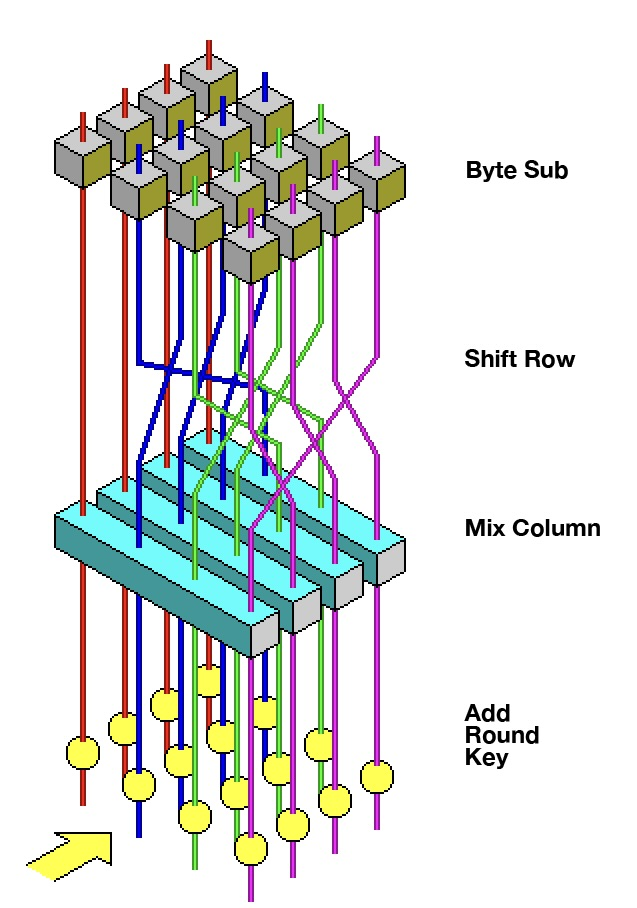
\includegraphics[width=\textwidth]{Chapter2/Figures/aes_round_function.jpeg}
        \caption{AES Round Function \cite{Wikipedia_AES_2024}}
        \label{fig:aes_round}
    \end{minipage}%
    \hfill
    \begin{minipage}{0.5\textwidth}
        \text{3. Middle rounds:}
        \begin{enumerate}
            \item $SubBytes$: each byte is substituted with another according to a lookup table (the SBox).
            \item $ShiftRows$: then, the last three rows of the substituted bytes are shifted cyclically.
            \item $MixColumns$: The four bytes in each column are then combined.
            \item $AddRoundKey$: finally, the round key is XOR-ed with each byte of the state (same as step 2).
        \end{enumerate}
        \vspace{0.5em}
        These middle rounds are executed $n$ times, depending on the key size:
        \begin{itemize}
            \item $n=10$ rounds for 128-bit keys
            \item $n=12$ rounds for 192-bit keys
            \item $n=14$ rounds for 256-bit keys
        \end{itemize}

    \end{minipage}
\end{figure}
The final output is our encrypted input text. AES has been heavily and publicly scrutinised for decades since its adoption by the U.S. government \cite{FIPS197} (aside from side-channel attacks, not technically a fault of the algorithm). It's also performant, as it can be implemented in-place with constant-time operations. And it's flexible, as multiple key-sizes are available and can be chosen based on an application's memory/time complexity constraints.

It's worth mentioning too that the decryption process essentially reverses the encryption process; but it uses inverse versions of the encryption steps, applied in a reverse order.

\subsection{Performing an AES encryption via OpenSSL}
An AES 256-bit CBC encryption of a text file can be performed via the open-source, OpenSSL library which implements SSL and TLS protocols for linux systems:

\ \\
\texttt{
openssl enc -aes-256-cbc -salt -in plaintext.txt -out encrypted.bin -k \\ MySecretKey -pbkdf2
}
\ \\

Where:
\begin{itemize}
    \item \texttt{-aes-256-cbc}: Specifies the encryption algorithm (AES-256 in CBC mode).
    \item \texttt{-salt}: Adds a salt to the password for added security.
    \item \texttt{-in plaintext.txt}: The input file to be encrypted.
    \item \texttt{-out encrypted.bin}: The output file where the encrypted data will be stored.
    \item \texttt{-k MySecretKey}: The key used for encryption.
    \item \texttt{-pbkdf2}: Uses PBKDF2 (Password-Based Key Derivation Function 2) for key generation, which is more secure than the default (A warning for deprecated key generation usage will appear if this is omitted (OpenSSL 3.3.1)).
\end{itemize}
Of course, the "\texttt{plaintext.txt}" file is only securely encrypted if the key is not made public.
\section{RISC-V Instruction Set Architecture}
RISC-V is an open-source Instruction Set Architecture (ISA) developed at the University of California, Berkeley in 2010 [1]. It aims to provide a modern, modular, and extensible ISA for a wide range of computing devices. The RISC-V ecosystem has grown rapidly, with major tech companies and startups adopting the architecture. As of 2024, RISC-V processors have made substantial progress in performance, though they still lag behind the most advanced x86 and ARM designs in high-performance applications. For instance, the SiFive Performance P670 core, announced in late 2022, claimed performance comparable to Arm Cortex-A77 cores from 2019 [2].

RISC-V's main advantage, is in it's open-sourceness and potential for customization. Many companies are leveraging RISC-V for specialized applications, such as AI accelerators, where the ability to add custom instructions can provide significant advantages [3]. While RISC-V is still maturing in the high-performance computing space, it has already found significant success in microcontrollers and embedded systems. As of 2023, RISC-V International reported that over 10 billion RISC-V cores have been shipped, primarily in microcontrollers and embedded devices [4]. As the ecosystem continues to evolve, with more software support and advanced implementations, RISC-V is poised to become an increasingly important player in the processor market across various computing domains.

\section{FPGAs}
\subsection{Softcore CPUs}

\subsection{Chosen Softcore CPU: VexRiscv}

\subsection{SpinalHDL}

\subsection{CPU Buses, Wishbone}

\subsection{VexRiscvSMP}

\section{Litex}

\subsection{Cores}

\subsection{Litex BIOS}

\subsection{Buildroot Linux}
\raggedbottom
